

\tikzset{every picture/.style={line width=0.45pt}} %set default line width to 0.75pt        

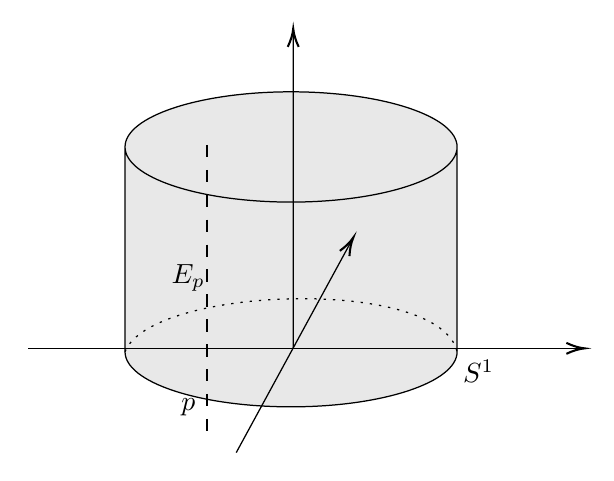
\begin{tikzpicture}[scale=0.8, x=0.75pt,y=0.75pt,yscale=-1,xscale=1]
%uncomment if require: \path (0,445); %set diagram left start at 0, and has height of 445

%Flowchart: Magnetic Disk [id:dp05785587446091456] 
\draw  [fill={rgb, 255:red, 232; green, 232; blue, 232 }  ,fill opacity=1 ] (298.5,110.04) -- (298.5,233.36) .. controls (298.5,251.7) and (253.73,266.56) .. (198.5,266.56) .. controls (143.27,266.56) and (98.5,251.7) .. (98.5,233.36) -- (98.5,110.04)(298.5,110.04) .. controls (298.5,128.38) and (253.73,143.25) .. (198.5,143.25) .. controls (143.27,143.25) and (98.5,128.38) .. (98.5,110.04) .. controls (98.5,91.71) and (143.27,76.84) .. (198.5,76.84) .. controls (253.73,76.84) and (298.5,91.71) .. (298.5,110.04) -- cycle ;
%Straight Lines [id:da047201416380546535] 
\draw    (40.25,231.34) -- (373.25,231.34) ;
\draw [shift={(375.25,231.34)}, rotate = 180] [color={rgb, 255:red, 0; green, 0; blue, 0 }  ][line width=0.75]    (10.93,-3.29) .. controls (6.95,-1.4) and (3.31,-0.3) .. (0,0) .. controls (3.31,0.3) and (6.95,1.4) .. (10.93,3.29)   ;
%Straight Lines [id:da32140623967458537] 
\draw    (165.5,294.09) -- (235.04,166.34) ;
\draw [shift={(236,164.59)}, rotate = 118.56] [color={rgb, 255:red, 0; green, 0; blue, 0 }  ][line width=0.75]    (10.93,-3.29) .. controls (6.95,-1.4) and (3.31,-0.3) .. (0,0) .. controls (3.31,0.3) and (6.95,1.4) .. (10.93,3.29)   ;
%Curve Lines [id:da7976987955408381] 
\draw  [dash pattern={on 0.84pt off 2.51pt}]  (98.5,233.36) .. controls (114,193.84) and (288,187.84) .. (298.5,233.36) ;
%Straight Lines [id:da639687396341936] 
\draw    (199.75,231.34) -- (199.8,40.84) ;
\draw [shift={(199.8,38.84)}, rotate = 90.01] [color={rgb, 255:red, 0; green, 0; blue, 0 }  ][line width=0.75]    (10.93,-3.29) .. controls (6.95,-1.4) and (3.31,-0.3) .. (0,0) .. controls (3.31,0.3) and (6.95,1.4) .. (10.93,3.29)   ;
%Straight Lines [id:da5733655963811695] 
\draw  [dash pattern={on 4.5pt off 4.5pt}]  (147.8,108.8) -- (147.8,281.8) ;

% Text Node
\draw (130.8,260.24) node [anchor=north west][inner sep=0.75pt]    {$p$};
% Text Node
\draw (125,179.4) node [anchor=north west][inner sep=0.75pt]    {$E_{p}$};
% Text Node
\draw (300.5,236.76) node [anchor=north west][inner sep=0.75pt]    {$S^{1}$};


\end{tikzpicture}